\chapter{Tổng quan}\label{chapter_overview}


\section{Chèn hình ảnh}

Hình \ref{icc_plot} minh họa chèn hình ảnh vào báo cáo.
 
\begin{center}
    \begin{figure}[h!]
    \begin{center}
     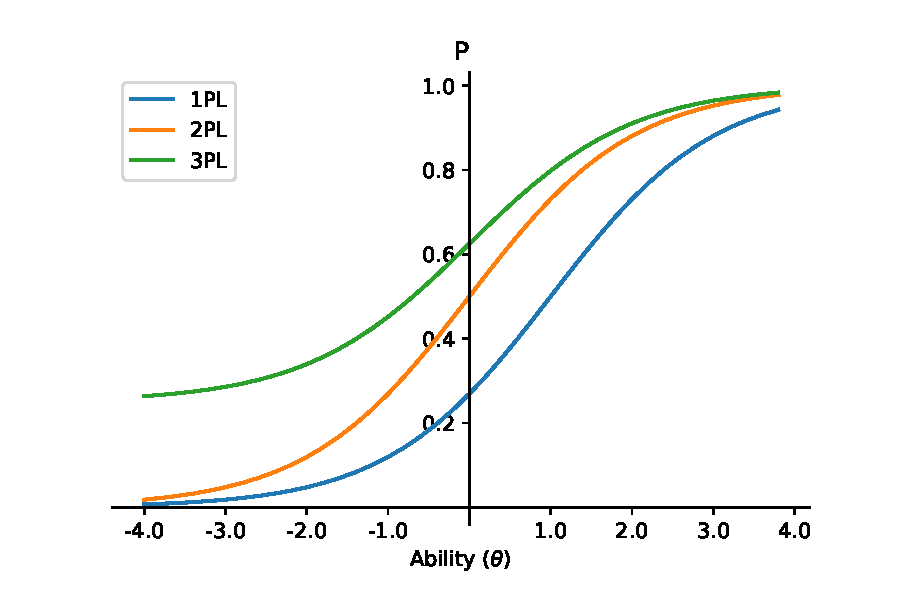
\includegraphics[scale=0.5]{figs/ICC_plots.pdf}
    \end{center}
    \caption{Một ví dụ về chèn hình ảnh.}
    \label{icc_plot}
    \end{figure}
\end{center}

\section{Chèn bảng}

\begin{center}
    \begin{table}
    \centering
    \caption{Ví dụ về tạo bảng trong \LaTeX. Tham khảo: \url{https://en.wikibooks.org/wiki/LaTeX/Tables}.}
        \begin{tabular}{ |l|l|l| }
        \hline
        \multicolumn{3}{ |c| }{Danh sách U23 Việt Nam tại Sea Games 31} \\
        \hline
        Thủ môn & GK & Nguyễn Văn Toản \\ \hline
        \multirow{4}{*}{Hậu vệ} & LB & Phan Tuấn Tài \\
         & DC & Bùi Hoàng Việt Anh \\
         & DC & Lê Văn Đô \\
         & RB & Lê Văn Xuân \\ \hline
        \multirow{3}{*}{Tiền vệ} & MC & Đỗ Hùng Dũng \\
         & MC & Nguyễn Hoàng Đức \\
         & MC & Dụng Quang Nho \\ \hline
        
        \multirow{2}{*}{Tiền đạo} & ST & Nhâm Mạnh Dũng \\
         & ST & Nguyễn Văn Tùng \\
         & FW & Nguyễn Tiến Linh \\
        \hline
        \end{tabular}
    
    \end{table}
\end{center}

\section{Chèn công thức toán học}

Công thức \ref{eq:InterTweetInteraction} thể hiện mức độ tương tác giữa hai tập $T_{j}^{P}$ và $T_{k}^{P}$.

\begin{align}
S_{j,k}^{P}=\frac{\sum_{t_{m}^{P}\in T_{j}^{P}}\sum_{t_{n}^{P}\in T_{k}^{P}}r\left(t_{m}^{P},t_{n}^{P}\right)}{|T_{j}^{P}||T_{k}^{P}|}\label{eq:InterTweetInteraction}
\end{align}

Để soạn thảo các công thức toán học được dễ dàng hơn, có thể sử dụng một phần mềm hỗ trợ nhập công thức theo dạng What You See Is What You Mean (WYSIWYM), chẳng hạn như \href{https://www.lyx.org/}{LyX}, sau đó copy LaTeX code vào file .tex (xem Hình \ref{lyx_example}), sẽ được kết quả như Công thức \ref{eq:ErrorFunction}.

\begin{center}
    \begin{figure}[h!]
    \begin{center}
     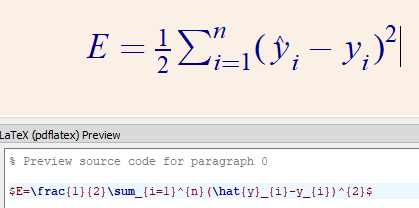
\includegraphics[scale=0.5]{figs/LyX.PNG}
    \end{center}
    \caption{Ví dụ cách soạn thảo công thức bằng LyX và copy sang file .tex.} 
    \label{lyx_example}
    \end{figure}
\end{center}

\begin{align}
E=\frac{1}{2}\sum_{i=1}^{n}(\hat{y}_{i}-y_{i})^{2}
\label{eq:ErrorFunction}
\end{align}



\section{Chèn mã nguồn}
Có thể sử dụng package minted để chèn mã nguồn vào báo cáo. Có thể chèn mã nguồn trực tiếp hoặc từ file có sẵn.

\noindent\textbf{Ví dụ 1:} Chèn mã nguồn trực tiếp.
\begin{minted}{C++}
#include<stdio.h>
int main()
{
	printf("Hello world!");
}
\end{minted}


\noindent\textbf{Ví dụ 2:} Chèn mã nguồn từ file. Đoạn mã nguồn sau đây được chèn từ file \path{code/XulyFileText.cpp}

\inputminted{c++}{code/XulyFileText.cpp}
\section{Biểu diễn giải thuật}
    \begin{algorithm}[H]
    \caption{Kiểm tra một số tự nhiên có phải số nguyên tố hay không}\label{prime_number_check}
    \hspace*{\algorithmicindent} \textbf{Input:} 
    Số tự nhiên \textbf{n}\\
    \hspace*{\algorithmicindent} \textbf{Output:} 
    True nếu \textbf{n} là số nguyên tố,
    False nếu \textbf{n} không phải số nguyên tố
    \begin{algorithmic}[1]
    \Function{isPrimeNumber}{n}
    \If {$n < 2$} \Return False
    \EndIf
    \For{$i \gets 2$ to $n/2$}
    \If{$n \% i == 0$} \Return False
    \EndIf
    \EndFor
    \State \Return True
    \EndFunction
    \end{algorithmic}
    \end{algorithm}


\section{Chèn chú thích vào cuối trang (footnote)}
Khi cần chèn một dòng chú thích vào cuối trang, sử dụng lệnh \textbf{footnote}\footnote{Đây là dòng chú thích}.




